\documentclass[a4paper,landscape,9pt]{article}

\usepackage[margin=1cm]{geometry}
\usepackage{fontspec}
\setmainfont{TeX Gyre Pagella}
\usepackage{unicode-math}
\setmathfont{TeX Gyre Pagella Math}

\usepackage{tikz}
\usetikzlibrary{arrows.meta,calc,positioning,shapes.geometric}
\usepackage{microtype}

\pagestyle{empty}
\setlength{\parindent}{0pt}
\setlength{\parskip}{0.25em}

\tikzset{
  node-d/.style={draw,fill=black,regular polygon,regular polygon sides=6,minimum size=7mm,inner sep=0pt,text=white,font=\tiny\bfseries},
  node-a/.style={draw,fill=black!70,regular polygon,regular polygon sides=3,minimum size=7mm,inner sep=0pt,text=white,font=\tiny\bfseries},
  node-t/.style={draw,circle,minimum size=7mm,inner sep=0pt,line width=0.4pt,font=\tiny},
  node-o/.style={draw,fill=black!15,rectangle,minimum size=7mm,inner sep=0pt,font=\tiny},
  node-i/.style={draw,diamond,minimum size=8mm,inner sep=0pt,line width=0.4pt,font=\tiny},
  impl/.style={-{Latex[length=1.2mm]},line width=0.3pt,black!80},
  exemp/.style={-{Latex[length=1.2mm]},line width=0.3pt,dashed,black!80},
  band/.style={font=\scriptsize\scshape,text=black!60},
  bandline/.style={draw,black!18,line width=0.3pt},
}

\begin{document}

\begin{center}
{\large\scshape Proposisjonsgraf, seksjon 7}\hspace{0.8em}{\itshape Forma viser kor langt omhugen rakk}
\end{center}

\vspace{-0.6em}

\begin{center}
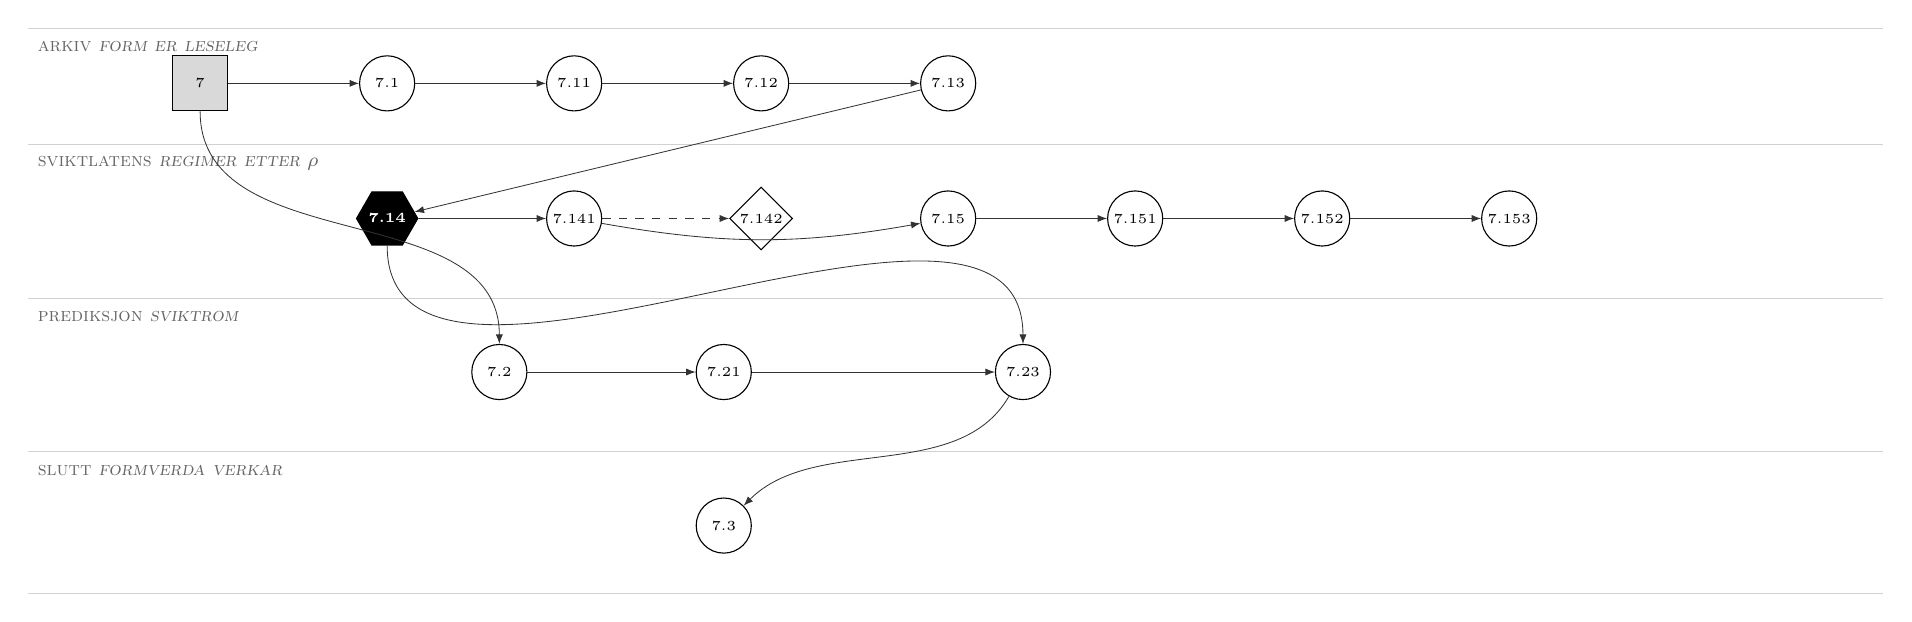
\begin{tikzpicture}[x=0.95cm,y=0.78cm]

  \draw[bandline] (-0.3, 0.6)  -- (24.5, 0.6);
  \draw[bandline] (-0.3, -1.3) -- (24.5, -1.3);
  \draw[bandline] (-0.3, -3.8) -- (24.5, -3.8);
  \draw[bandline] (-0.3, -6.3) -- (24.5, -6.3);
  \draw[bandline] (-0.3, -8.6) -- (24.5, -8.6);

  \node[band,anchor=west] at (-0.3, 0.3)  {arkiv  \itshape form er leseleg};
  \node[band,anchor=west] at (-0.3, -1.6) {sviktlatens  \itshape regimer etter $\rho$};
  \node[band,anchor=west] at (-0.3, -4.1) {prediksjon  \itshape sviktrom};
  \node[band,anchor=west] at (-0.3, -6.6) {slutt  \itshape formverda verkar};

  % BAND 1: arkiv (form er leseleg)
  \node[node-o] (p7)     at (2, -0.3)    {7};
  \node[node-t] (p71)    at (4.5, -0.3)  {7.1};
  \node[node-t] (p711)   at (7, -0.3)    {7.11};
  \node[node-t] (p712)   at (9.5, -0.3)  {7.12};
  \node[node-t] (p713)   at (12, -0.3)   {7.13};
  \draw[impl] (p7)   -- (p71);
  \draw[impl] (p71)  -- (p711);
  \draw[impl] (p711) -- (p712);
  \draw[impl] (p712) -- (p713);

  % BAND 2: sviktlatens (nytt: \rho-regimer)
  \node[node-d] (p714)   at (4.5, -2.5)  {7.14};
  \node[node-t] (p7141)  at (7, -2.5)    {7.141};
  \node[node-i] (p7142)  at (9.5, -2.5)  {7.142};
  \node[node-t] (p715)   at (12, -2.5)   {7.15};
  \node[node-t] (p7151)  at (14.5, -2.5) {7.151};
  \node[node-t] (p7152)  at (17, -2.5)   {7.152};
  \node[node-t] (p7153)  at (19.5, -2.5) {7.153};
  \draw[impl] (p713)   -- (p714);
  \draw[impl] (p714)   -- (p7141);
  \draw[exemp] (p7141) -- (p7142);
  \draw[impl] (p7141)  to[bend right=10] (p715);
  \draw[impl] (p715)   -- (p7151);
  \draw[impl] (p7151)  -- (p7152);
  \draw[impl] (p7152)  -- (p7153);

  % BAND 3: predikert sviktrom (rein deskriptiv)
  \node[node-t] (p72)    at (6, -5)      {7.2};
  \node[node-t] (p721)   at (9, -5)      {7.21};
  \node[node-t] (p723)   at (13, -5)     {7.23};
  \draw[impl] (p7)    to[out=-90,in=90,looseness=1.0] (p72);
  \draw[impl] (p72)   -- (p721);
  \draw[impl] (p721)  -- (p723);
  \draw[impl] (p714)  to[out=-90,in=90,looseness=0.9] (p723);

  % BAND 4: slutt
  \node[node-t] (p73)    at (9, -7.5)    {7.3};
  \draw[impl] (p723)  to[out=-120,in=45,looseness=0.9] (p73);

\end{tikzpicture}
\end{center}

\vspace{-0.2em}

\hrule

\vspace{0.4em}

\begin{minipage}[t]{0.325\textwidth}
{\scshape\small Lesing ovanfrå}

Rota \emph{7} seier at forma viser kor langt omhugen rakk. Band 1 etablerer \textbf{arkiv-tesen}: \emph{7.1} seier at forma er eit leseleg arkiv over kompromissets dimensjonalitet. \emph{7.11} til \emph{7.13} gjev han presisjon: arkivet ber signaturen av blindskapen, to former under ulik omhug skil seg langs det eine såg og det andre ikkje, og arkivet er faktum, ikkje skulding.

Band 2 innfører \textbf{sviktlatensen} $\rho_i = \tau(X_i)/\tau(A)$ (\emph{7.14}): ratioen mellom responstida langs aksen og agentens prediksjonshorisont. \emph{7.141} definerer tre regimer (internalisert, leseleg, strukturelt usynleg); \emph{7.142} illustrerer (ergonomi: $\rho\sim 10$; eingongskopp: $\rho\sim 10^6$). Resten av bandet (\emph{7.15}--\emph{7.153}) er meta-teoremet om at teorien må predikere sviktsignatur, ikkje berre katalogisere han.
\end{minipage}\hfill
\begin{minipage}[t]{0.325\textwidth}
{\scshape\small Lesing nedover}

Band 3 er no \emph{rein deskriptiv}. Endringsplanen flytta dei tre normative postulata (tidlegare 7.2, 7.202, 7.22) ut av traktaten og til etterordet/breva, der den normative tiltalen alltid har budd. Det som står att:

\emph{7.2} seier at designhandlinga har empirisk verknad på andre agentars generative modellar. \emph{7.21} seier at ei form designa under trong omhug etterlèt signatur langs dei urepresenterte aksane. \emph{7.23} definerer \textbf{det predikerte sviktrommet}: vektoren $(C(A)\setminus\omega(A))$ vekta med $\{\rho_i\}$. Modellen predikerer; agenten avgjer relevans.

Band 4 er éin node. \emph{7.3} er traktaten sin coda.
\end{minipage}\hfill
\begin{minipage}[t]{0.325\textwidth}
{\scshape\small Strukturelle innsikter}

\emph{F2 løyst.} Normativt innhald er flytta ut av modellen; Hume si giljotin står urørt. Modellen er rein prediksjon; bruken er der valet ligg.

\emph{Ingen postulat.} Frå tre til null. Seksjonen er no kategorisert som \emph{karakterisering} på lik linje med 3 og 4. Sjangerinndelinga kollapsar frå fire til tre.

\emph{Ny definisjon.} \emph{7.14} (sviktlatensen) er seksjonens einaste definisjon. Ho gjev prediksjonen kvantitativ struktur.

\emph{Kompositorisk symmetri.} \emph{7.23} speglar \emph{1.131} som avslutningsteorem; \emph{7.3} speglar \emph{1}: formverda som det som verkar, mot formverda som det som er tilfelle.

\emph{Ingen sjanger "normativ karakterisering".} Den fjerde sjangeren er eliminert; symmetrien i atlaset er restituert.
\end{minipage}

\end{document}
